\documentclass{beamer}

\usetheme{Madrid}
\usepackage[english]{babel}
\usepackage[utf8x]{inputenc}
\usepackage[T1]{fontenc}
\usepackage{url,alltt,xspace,amsmath,txfonts,helvet}
\usepackage{lmodern}
\usepackage{listings}
\usepackage{graphicx}
\let\Tiny=\tiny

\definecolor{uib}{rgb}{0,.33,.45}
\definecolor{green}{rgb}{.47,.68,0}
\definecolor{orange}{rgb}{.85,.35,0}
\definecolor{red}{rgb}{.67,.0,0}
\definecolor{darkuib}{rgb}{0,.165,.225}
\definecolor{darkgreen}{rgb}{.235,.34,0}
\definecolor{reallydarkgreen}{rgb}{.117,.17,0}
\definecolor{darkorange}{rgb}{.425,.175,0}
\definecolor{darkred}{rgb}{.333,.0,0}
\setbeamercolor{structure}{fg=green!80!black}

\title{CoffeeW8 - Coffee forecast}
\author{Alexander Hoem Rosbach}

\pgfdeclareimage[height=7ex]{bldl}{images/logo-with-text.pdf}
\pgfdeclareimage[height=8.5ex]{iiuib}{images/uib-logo-flushright.pdf}
\date{\today}

\institute[2012]{Master student, UiB/BLDL}

\begin{document}

\logo{\parbox{\linewidth}{\pgfuseimage{bldl}\hspace*{\fill}\pgfuseimage{iiuib}\hspace*{3em}}}
\frame{\titlepage}
\logo{}

\begin{frame}
    \frametitle{Outline}
    \tableofcontents
\end{frame}

\section{Project description}
\begin{frame}
    \frametitle{CoffeeW8}
    \centerline{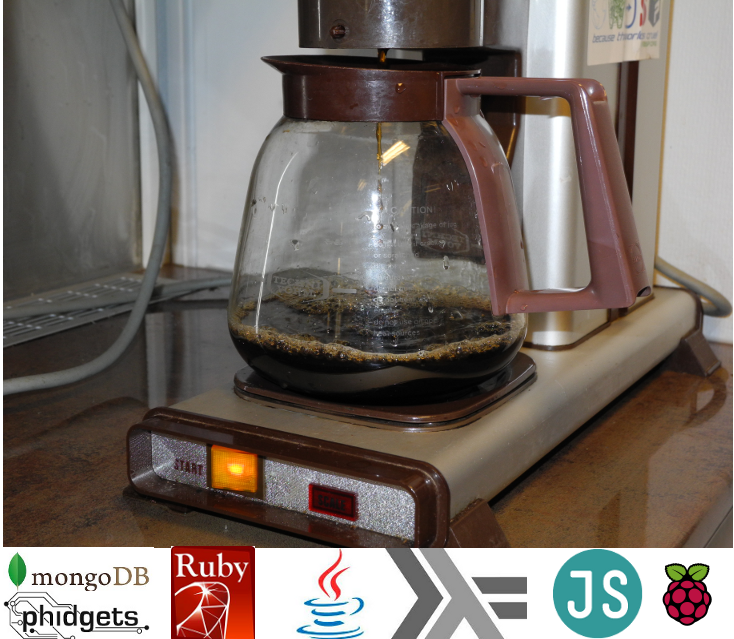
\includegraphics[scale=1.5]{images/project.png}}
\end{frame}
\subsection{Motivation}
\begin{frame}
    \frametitle{Motivation}
    \begin{itemize}
        \item Forecasts
        \item Current status
        \item Sensor system
        \item Fun
        \item \url{http://www.github.com/veiset/CoffeeW8}
    \end{itemize}
\end{frame}

\subsection{Modules}
\begin{frame}
    \frametitle{Modules}
    \begin{itemize}
        \item Database - Haskell
        \item Web - Ruby
        \item Reader - Java
    \end{itemize}
\end{frame}

\section{Reader module}
\begin{frame}
    \frametitle{Reader module}
    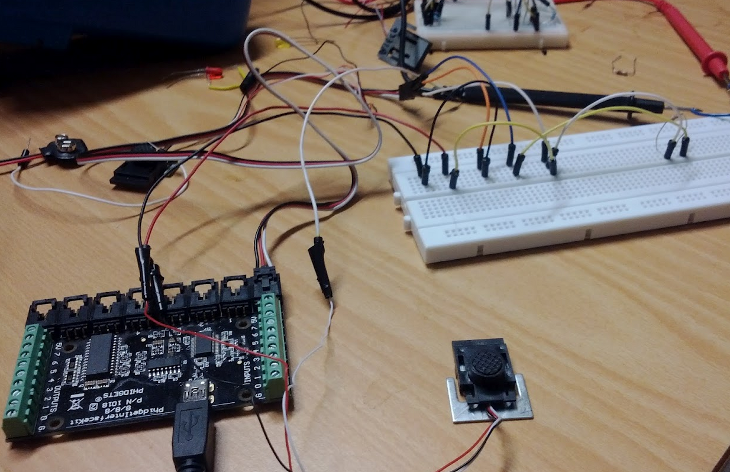
\includegraphics[scale=0.46]{images/wsensor.png}
\end{frame}
\subsection{Specification}
\begin{frame}
    \frametitle{Specification}
    \begin{itemize}
        \item Hardware: Low-end (and low-cost) small SBC device (R$\pi$)
        \item Low memory/cpu resource requirements
        \item Read and buffer sensor data
        \item REST API
        \item Placement: close to the coffee machine
    \end{itemize}
\end{frame}

\subsection{Implementation}
\begin{frame}
    \frametitle{Implementation}
    \begin{itemize}
        \item Restlet framework (\url{www.restlet.org})
        \item Data as json
        \item Phidget API (Sensors)
        \item Cyclic buffer (Ring buffer)
    \end{itemize}
\end{frame}

\subsection{UnixtimeRingBuffer - data structure}
\begin{frame}
    \frametitle{UnixtimeRingBuffer - data structure}
    \begin{itemize}
        \item Stores data entries (CoffeeState entity)
        \item Must maintain a Total Order (JaxT requirement)
    \end{itemize}
\end{frame}

\subsection{CoffeeState - data entity}
\begin{frame}
    \frametitle{CoffeeState - data entity}
    \begin{itemize}
        \item Stores data pair <unixtime, weight>
        \item \emph{unixtime} is identity
%        \item Overrides \emph{equals} relation and \emph{hashcode}
%        \item Implements comparable
    \end{itemize}
\end{frame}

\section{JaxT}
\begin{frame}
    \frametitle{Jaxt for Reader}
    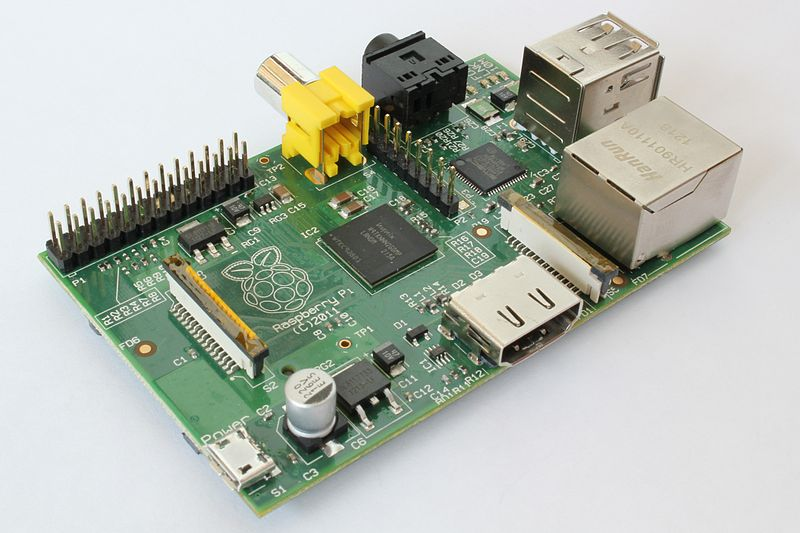
\includegraphics[scale=0.46]{images/rpi.jpg}
\end{frame}

\subsection{Approach}
\begin{frame}
    \frametitle{Approach}
    \begin{itemize}
        \item Code first
        \item Then requirements (axioms)
        \item Improve implementation
        \item More requirements
    \end{itemize}
\end{frame}

\subsection{Discoveries}
\begin{frame}
    \frametitle{Discoveries}
    \begin{itemize}
        \item UnixtimeRingBuffer did not implement a total order
        \item UnixtimeRingBuffer methods had some bugs
        \item CoffeeState needed a binary relation, \emph{newerThan} (transitive, irreflexive, asymmetric)
    \end{itemize}
\end{frame}



\end{document}
